\chapter{UrbanSim}

\section{Design Objectives and Key Features}

UrbanSim is an urban simulation system developed over the past
several years to better inform deliberation on public choices with
long-term, significant effects\footnote{This chapter draws in part
on reference \cite{waddell-brail-book-2001}}.  The principal motivation 
was that the urban environment
is complex enough that it is not feasible to anticipate the effects
of alternative courses of action without some form of analysis that
could reflect the cause and effect interactions that could have both
intended and possibly unintended consequences.

Consider a highway expansion project, for example.  Traditional civil engineering training from the mid 20th century suggested that the problem was a relatively simple one: excess demand meant that vehicles were forced to slow down, leading to congestion bottlenecks.  The remedy was seen as easing the bottleneck by adding capacity, thus restoring the balance of capacity to demand.  Unfortunately, as Downs (2004) has articulately explained, and most of us have directly observed, once capacity is added, it rather quickly gets used up, leading some to conclude that `you can't build your way out of congestion'. The reason things are not as simple as the older engineering perspective would have predicted is that individuals and organizations adapt to changing circumstances.  Once the new capacity is available, initially vehicle speeds do increase, but this drop in the time cost of travel on the highway allows drivers taking other routes to change to this now-faster route, or to change their commute to work from a less-convenient shoulder of the peak time to a mid-peak time, or switching from transit or car-pooling to driving alone, adding demand at the most desired time of the day for travel.  Over the longer-term, developers take advantage of the added capacity to build new housing and commercial and office space, households and firms take advantage of the accessibility to move farther out where they can acquire more land and sites are less expensive.  In short, the urban transportation system is in a state of dynamic equilibrium, and when you perturb the equilibrium, the system, or more accurately, all the agents in the system, react in ways that tend to restore equilibrium.  If there are faster speeds to be found to travel to desired destinations, people will find them.

The highway expansion example illustrates a broader theme: urban systems that include the transportation system, the housing market, the labor market (commuting), and other real estate markets for land, commercial, industrial, warehouse, and office space - are closely interconnected - much like the global financial system.  An action taken in one sector ripples through the entire system to varying degrees, depending on how large an intervention it is, and what other interventions are occurring at the same time.
This brings us to a second broad theme: interventions are rarely coordinated with each other, and often are conflicting or have a compounding effect that was not intended.  This pattern is especially true in metropolitan areas consisting of many local cities and possibly multiple counties - each of which retain control of land use policies over a fraction of the metropolitan area, and none of which have a strong incentive, nor generally the means, to coordinate their actions.  It is more often the case that local jurisdictions are taking actions in strategic ways that will enhance their competitive position for attracting tax base-enhancing development and residents.  It is also systematically the case that transportation investments are evaluated independently of land use plans and the reactions of the real estate market.

UrbanSim was designed to attempt to reflect the interdependencies in dynamic urban systems, focusing on the real estate market and the transportation system, initially, and on the effects of individual interventions, and combinations of them, on patterns of development, travel demand, and household and firm location.  Some goals that have shaped the design of UrbanSim, and some that have emerged through the past several years of seeing it tested in the real world, are the following:

Outcome Goals:
\squishlist
\item Enable a wide variety of stakeholders (planners, public agencies, citizens and advocacy groups) to explore the potential consequences of alternative public policies and investments using credible, unbiased analysis.
\item Facilitate more effective democratic deliberation on contentious public actions regarding land use, transportation and the environment, informed by the potential consequences of alternative courses of action that include long-term cumulative effects on the environment, and distributional equity considerations.
\item Make it easier for communities to achieve a common vision for the future of the community and its broader environment, and to coordinate their actions to produce outcomes that are consistent with this vision.
\squishend

Implementation Goals for UrbanSim:
\squishlist
\item Create an analytical capacity to model the cause and effect interactions within local urban systems that are sufficiently accurate and sensitive to policy interventions to be a credible source for informing deliberations.
\item Make the model system credible by avoiding bias in the models though simplifying assumptions that obscure or omit important cause-effect linkages at a level of detail needed to address stakeholder concerns.
\item Make the model design behaviorally clear in terms of representing agents, actions, and cause - effect interactions in ways that can be understood by non-technical stakeholders, while making the statistical methods used to implement the model scientifically robust.
\item Make the model system open, accessible and transparent, by adopting an Open Source licensing approach and releasing the code and documentation on the web.
\item Encourage the development of a collaborative approach to development and extension of the system, both through open source licensing and web access, and by design choices and supporting organizational activities.
\item Test the system extensively and repeatedly, and continually improve it by incorporating lessons learned from applications, and from new advances in methods for modeling, statistical analysis, and software development.
\squishend

The original design of UrbanSim adopted several elements to address these implementation goals, and these have remained foundational in the development of the system over time.  These design elements include:

\squishlist
\item The representation of individual agents: initially households and firms, and later, persons and jobs.
\item The representation of the supply and characteristics of land and of real estate development, at a fine spatial scale: initially a mixture of parcels and zones, later gridcells of user-specified resolution.
\item   The adoption of a dynamic perspective of time, with the simulation proceeding in annual steps, and the urban system evolving in a path dependent manner.
\item   The use of real estate markets as a central organizing focus, with consumer choices and supplier choices explicitly represented, as well as the resulting effects on real estate prices.  The relationship of agents to real estate tied to specific locations provided a clean accounting of space and its use.
\item   The use of standard discrete choice models to represent the choices made by households and firms and developers (principally location choices).  This has relied principally on the traditional Multinomial Logit (MNL) specification, to date.
\item   Integration of the urban simulation system with existing transportation model systems, to obtain information used to compute accessibilities and their influence on location choices, and to provide the raw inputs to the travel models.
\item   The adoption of an Open Source licensing for the software, written originally in Java, and recently reimplemented using the Python language.  The system has been updated and released continually on the web since 1998 at www.urbansim.org.
\squishend

The basic features of the UrbanSim model and software implementation are highlighted in Table \ref{tab:key-features}.  The model is unique in that it departs from prior operational land use models based on cross-sectional, equilibrium, aggregate approaches to adopt an approach that models individual households, jobs, buildings and parcels (or gridcells), and their changes from one year to the next as a consequence of economic changes, policy interventions, and market interactions .

\begin{table}[htp]
\caption{Key Features of UrbanSim}
\label{tab:key-features}
\begin{center}
\begin{tabular}{ p{1.5in}  p{4.4in}  }
\toprule[1.5pt]
\multirow{8}{1.5in}{Key Features of the UrbanSim
Model System} &  $\bullet$   The model simulates the key decision makers and
choices impacting urban development; in particular, the mobility and
location choices of households and businesses, and the development
choices of developers\\
%\cmidrule{2-2}
&  $\bullet$   The model explicitly accounts for land, structures (houses and commercial buildings), and occupants (households and businesses)\\
%\cmidrule{2-2}
&  $\bullet$   The model simulates urban development as a dynamic process over time and space, as opposed to a cross-sectional or equilibrium approach\\
%\cmidrule{2-2}
&  $\bullet$   The model simulates the land market as the interaction of demand (locational preferences of businesses and households) and supply (existing vacant space, new construction, and redevelopment), with prices adjusting to clear market\\
%\cmidrule{2-2}
& $\bullet$    The model incorporates governmental policy assumptions explicitly, and evaluates policy impacts by modeling market responses\\
%\cmidrule{2-2}
& $\bullet$    The model is based on random utility theory and uses logit models for the implementation of key demand components\\
%\cmidrule{2-2}
& $\bullet$    The model is designed for high levels of spatial and activity disaggregation, with a zonal system identical to travel model zones\\
%\cmidrule{2-2}
& $\bullet$    The model presently addresses both new development and redevelopment, using parcel-level detail\\
\midrule
\multirow{8}{1,5in}{Key Features of the UrbanSim Software Implementation}
&  $\bullet$   The model and user interface is currently compatible with Windows, Linux, Apple OS X, and other platforms supporting Python\\
%\cmidrule{2-2}
& $\bullet$  The software is implemented in the Open Platform for Urban Simulation (Opus)\\
%\cmidrule{2-2}
& $\bullet$  The software is Open Source, using the GPL license\\
%\cmidrule{2-2}
& $\bullet$  The system is downloadable from the web at www.urbansim.org\\
%\cmidrule{2-2}
&  $\bullet$   The user interface focuses on configuring the model system, managing data, running and evaluating scenarios\\
%\cmidrule{2-2}
& $\bullet$    The model is implemented using object-oriented programming to maximize software flexibility\\
%\cmidrule{2-2}
&  $\bullet$   The model inputs and results can be displayed using ArcGIS or other GIS software such as PostGIS\\
%\cmidrule{2-2}
&  $\bullet$   Model results are written to binary files, but can be exported to database management systems, text files, or geodatabases\\
\bottomrule
\end{tabular}
\end{center}
\end{table}

\section{Model System Design}

The components of UrbanSim are models acting on the objects in Figure
\ref{fig:dataflow}, simulating the real-world actions of agents acting in the urban system.  Developers construct new buildings or redevelop existing ones.  Buildings are located on land parcels that have particular characteristics such as value, land use, slope, and other environmental characteristics.  Governments set policies that regulate the use of land, through the imposition of land use plans, urban growth boundaries, environmental regulations, or through pricing policies such as development impact fees.  Governments also build infrastructure, including transportation infrastructure, which interacts with the distribution of activities to generate patterns of accessibility at different locations that in turn influence the attractiveness of these sites for different consumers.  Households have particular characteristics that may influence their preferences and demands for housing of different types at different locations.  Businesses also have preferences that vary by industry and size of business (number of employees) for alternative building types and locations.

These urban actors and processes are implemented in model components that are connected through the software implementation shown in Figure \ref{fig:dataflow}. The diagram reflects the interaction between the land use and travel model systems, and between the land use model and the GIS used for data preparation and visualization.

\begin{figure}[htp]
\begin{center}
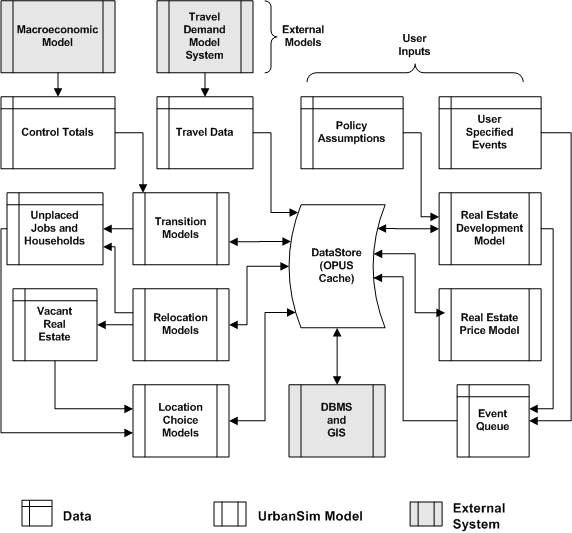
\includegraphics[scale=0.7]{graphics/flow-2008.png}
\end{center}
\caption{UrbanSim Model Components and Data Flow}
\label{fig:dataflow}
\end{figure}

UrbanSim predicts the evolution of these objects and their characteristics over time, using annual steps to predict the movement and location choices of businesses and households, the development activities of developers, and the impacts of governmental policies and infrastructure choices.  The land use model is interfaced with a metropolitan travel model system to deal with the interactions of land use and transportation. Access to opportunities, such as employment or shopping, are measured by the travel time or cost of accessing these opportunities via all available modes of travel.

The data inputs and outputs for operating the UrbanSim model are shown in Table \ref{tab:inputs-outputs}.  Developing the input database is challenging, owing to its detailed data requirements.  A GIS is required to manage and combine these data into a form usable by the model, and can also be used to visualize the model results.  Once the database is compiled, the model equations must be calibrated and entered into the model.  A final step before actual use of the model is a validation process that tests the operation of the model over time and makes adjustments to the dynamic components of the model.  The steps of data preparation, model estimation, calibration and validation will be addressed in later chapters.  In the balance of this chapter the design and specification of UrbanSim, using the most recent parcel-based approach used in the Puget Sound, is presented in more detail.

\begin{table}[htp]
\caption{Data Inputs and Outputs of UrbanSim}
\label{tab:inputs-outputs}
\begin{center}
\begin{tabular}{ p{1.5in}  p{4.4in}  }
%\addlinespace
\toprule[1.5pt]
\multirow{9}{1.5in}{UrbanSim Inputs}
&   $\bullet$ Employment data, in the form of geocoded business establishments\\
%\cmidrule{2-2}
&   $\bullet$ Household data, merged from multiple census sources\\
 %\cmidrule{2-2}
&   $\bullet$  Parcel database, with acreage, land use, housing units, nonresidential square footage, year built, land value, improvement value, city and county\\
 %\cmidrule{2-2}
&   $\bullet$  City and County General Plans\\
 %\cmidrule{2-2}
&   $\bullet$  GIS Overlays for environmental features such as wetlands, floodways, steep slopes, or other sensitive or regulated lands\\
 %\cmidrule{2-2}
&   $\bullet$  Traffic Analysis Zones\\
 %\cmidrule{2-2}
&   $\bullet$   GIS Overlays for any other planning boundaries\\
 %\cmidrule{2-2}
&   $\bullet$  Travel Model outputs\\
 %\cmidrule{2-2}
&  $\bullet$   Development Costs \\
\midrule
\multirow{6}{1.5in}{UrbanSim Outputs (by Building, Parcel or Gridcell), Generally Summarized by Zone}
& $\bullet$    Households by income, age, size, and presence of children\\
 %\cmidrule{2-2}
& $\bullet$    Employment by industry and land use type\\
%\cmidrule{2-2}
& $\bullet$    Acreage by land use\\
 %\cmidrule{2-2}
& $\bullet$    Dwelling units by type\\
 %\cmidrule{2-2}
& $\bullet$    Square feet of nonresidential space by type\\
 %\cmidrule{2-2}
& $\bullet$    Real estate prices\\
\midrule
\multirow{4}{1.5in}{Travel Model Outputs (Zone-to-Zone) Used in UrbanSim}
& $\bullet$    Travel time by mode by time of day by purpose\\
 %\cmidrule{2-2}
& $\bullet$  Trips by mode by time of day by purpose\\
 %\cmidrule{2-2}
& $\bullet$    Composite utility of travel using all modes by purpose \\
%\cmidrule{2-2}
& $\bullet$  Generalized costs (time + time equivalent of tolls) by purpose \\
\bottomrule
\end{tabular}
\end{center}
\end{table}

\section{Policy Scenarios}

UrbanSim is designed to simulate and evaluate the potential effects of multiple scenarios.  We use the term scenario in the context of UrbanSim in a very
specific way: a scenario is a combination of input data and assumptions to the model system, including macroeconomic assumptions regarding the growth of population and employment in the study area, the configuration of the transportation system assumed to be in place in specific future years, and
general plans of local jurisdictions that will regulate the types of development allowed at each location.

In order to facilitate comparative analysis, a model user such as a Metropolitan Planning Organization will generally adopt a specific scenario as a base of comparison or all other scenarios.  This base scenario is generally referred to as the `baseline' scenario, and this is usually based on the adopted or most
likely to be adopted regional transportation plan, accompanied by the most likely assumptions regarding economic growth and land use policies.  Once a  scenario is created, it determines several inputs to UrbanSim:

\squishlist
\item Control Totals: data on the aggregate amount of population and employment, by type, to be assumed for the region.
\item Travel Data: data on zone to zone travel characteristics, from the travel model.
\item Land Use Plan: data on general plans, assigned to individual parcels.
\item Development Constraints: a set of rules that interpret the general plan codes, to indicate the allowed land use types and density ranges on each parcel.
\squishend

\section{Discrete Choice Models}
\label{sec:discrete-choice}

UrbanSim makes extensive use of models of individual choice.  
A pathbreaking approach to modeling individual actions using discrete
choice models emerged in the 1970's, with the pioneering work of
McFadden on Random Utility Maximization theory
\cite{mcfadden-1974,mcfadden-1981}. This approach derives a model of
the probability of choosing among a set of available alternatives
based on the characteristics of the chooser and the attributes of
the alternative, and proportional to the relative utility that the
alternatives generate for the chooser. Maximum likelihood and
simulated maximum likelihood methods have been developed to estimate
the parameters of these choice models from data on revealed or
stated preferences, using a wide range of structural specifications
(see \cite{train-book-2003}). Early application of these models were
principally in the transportation field, but also included work on
residential location choices
\cite{quigley-eer-1976,lerman-trr-1977,mcfadden-1978}, and
on residential mobility \cite{clark-vanlierop-1986}.

Let us begin with an example of a simple model of households choosing among
alternative locations in the housing market, which we index by
$i$. For each agent, we assume that each alternative $i$ has
associated with it a utility $U_i$ that can be separated into a
systematic part and a random part:
\begin{equation}
    U_i = V_i + \epsilon_i,
    \label{eq:utility}
\end{equation}
%$V_i = \vk{\beta}\cdot\vk{x}_i$
where $V_i = \beta\cdot {x}_i$ is a linear-in-parameters
function, $\beta$ is a vector of $k$ estimable coefficients,
$x_i$ is a vector of observed, exogenous, independent
alternative-specific variables that may be interacted with the
characteristics of the agent making the choice, and $\epsilon_i$
is an unobserved random term. Assuming the unobserved term in
(\ref{eq:utility}) to be distributed with a Gumbel distribution
leads to the  widely used multinomial logit model
\cite{mcfadden-1974,mcfadden-1981}:
\begin{equation}
    P_i = \frac{\mathrm{e}^{V_i}}{\sum_j \mathrm{e}^{V_j}},
    \label{eq:mnl}
\end{equation}
where $j$ is an index over all possible alternatives. The
estimable coefficients of (\ref{eq:mnl}), $\beta$, are
estimated with the method of maximum likelihood (see for example
\cite{greene-2002}).

The denominator of the equation for the choice model has a particular
significance as an evaluation measure.  The log of this denominator
is called the \emph{logsum}, or composite utility, and it summarizes
the utility across all the alternatives.  In the context of a choice of
mode between origins and destinations, for example, it would summarize
the utility (disutility) of travel, considering all the modes connecting the
origins and destinations.  It has theoretical appeal as an evaluation
measure for this reason.  In fact, the logsum from the mode choice
model can be used as a measure of accessibility.

\begin{figure}[htp]
\center
 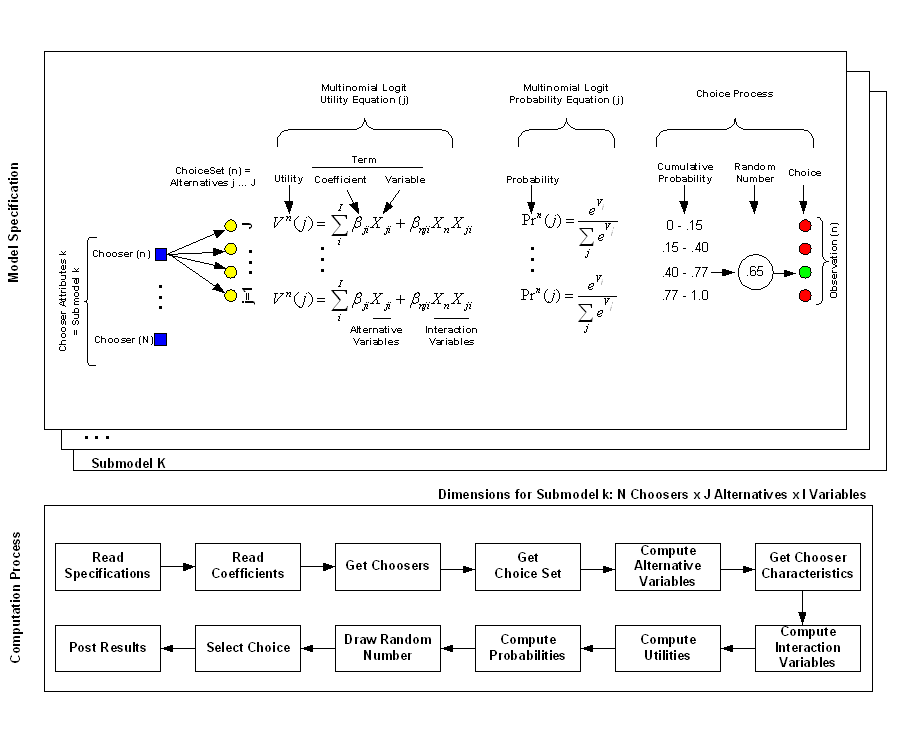
\includegraphics[width=6.5in]
 {graphics/ChoiceProcess.png}
\caption{Computation Process in UrbanSim Choice Models}
\label{fig:choiceprocess}
\end{figure}

Choice models are implemented in UrbanSim in a modular way, to allow flexible specification of models
to reflect a wide variety of choice situations.  Figure \ref{fig:choiceprocess} shows the process both in the form
of the equations to be computed, and from the perspective of the tasks implemented as methods in software.

For each model component within the UrbanSim model system, the
choice process proceeds as shown in Figure
\ref{fig:choiceprocess}. The first steps of the model read the
relevant model specifications and data.  Then a choice set is
constructed for each chooser.  Currently this is done using random
sampling of alternatives, which has been shown to generate consistent, though not
efficient, estimates of model parameters \cite{ben-akiva-lerman-1987}.

The choice step in this algorithm warrants further explanation.  Choice models predict choice probabilities, not choices.
In order to predict choices given the predicted probabilities, we require an algorithm to select a specific choice outcome.
A tempting approach would be to select the alternative with the maximum probability, but unfortunatelty this strategy
would have the effect of selecting only the dominant outcome, and less frequent alternatives would be completely
eliminated.  In a mode choice model, for illustration, the transit mode would disappear, since the probability of choosing
an auto mode is almost always higher than that of choosing transit.  Clearly this is not a desirable or realistic outcome.
In order to address this problem, the choice algorithm used for choice models uses a sampling approach.  As illustrated in Figure
\ref{fig:choiceprocess}, a choice outcome can be selected by sampling a random number from the uniform distribution in the range
0 to 1, and comparing this random draw to the cumulative probabilities of the alternatives.  Whichever alternative the sampled
random number falls within is the alternative that is selected as the `chosen' one.  This algorithm has the property that it
preserves in the distribution of choice outcomes a close approximation of the original probability distribution, especially
as the sample size of choosers becomes larger.

One other choice context is worth noting.  In some situations, the availability of alternatives may be constrained.  If the limit on availability
is entirely predictable, such as a budget constraint eliminating expensive options, or a zero-car household being unable to use the drive-alone
mode, this is straightforward to handle, by eliminating the alternatives from the choice set for those choosers.  In other situations, however, the
solution is not so straightforward.  In the case where alternatives may be unavailable because many other agents wish to choose them, the problem
is that the alternative may be unavailable due to the endogenous congestion of alternatives.  The effect of this is potentially significant, since it
may cause parameters estimated in a choice model to confuse, or confound, the effects of preferences with the effects of constraints.  Fortunately,
an estimation method has been developed to account for this problem \cite{depalma-jue-2007}.
